% Template pour faire aide-mémoire
\documentclass[10pt, french]{article}

%% -----------------------------
%% Préambule
%% -----------------------------
% !TEX encoding = UTF-8 Unicode
% LaTeX Preamble for all cheatsheets
% Author : Gabriel Crépeault-Cauchon

% HOW-TO : copy-paste this file in the same directory as your .tex file, and add in your preamble the next command right after you have specified your documentclass : 
% \input{preamble-cheatsht.tex}
% ---------------------------------------------
% ---------------------------------------------

% Extra note : this preamble creates document that are meant to be used inside the multicols environment. See the documentation on internet for further information.

%% -----------------------------
%% Encoding packages
%% -----------------------------
\usepackage[utf8]{inputenc}
\usepackage[T1]{fontenc}
\usepackage{babel}
\usepackage{lmodern}

%% -----------------------------
%% Variable definition
%% -----------------------------
\def\auteur{Gabriel Crépeault-Cauchon / Nicholas Langevin}
\def\BackgroundColor{white}

%% -----------------------------
%% Margin and layout
%% -----------------------------
% Determine the margin for cheatsheet
\usepackage[landscape, hmargin=1cm, vmargin=1.7cm]{geometry}
\usepackage{multicol}

% Remove automatic indentation after section/subsection title.
\setlength{\parindent}{0cm}

% Save space in cheatsheet by removing space between align environment and normal text.
\usepackage{etoolbox}
\newcommand{\zerodisplayskips}{%
  \setlength{\abovedisplayskip}{0pt}%
  \setlength{\belowdisplayskip}{0pt}%
  \setlength{\abovedisplayshortskip}{0pt}%
  \setlength{\belowdisplayshortskip}{0pt}}
\appto{\normalsize}{\zerodisplayskips}
\appto{\small}{\zerodisplayskips}
\appto{\footnotesize}{\zerodisplayskips}

%% -----------------------------
%% URL and links
%% -----------------------------
\usepackage{hyperref}
\hypersetup{colorlinks = true, urlcolor = gray!70!white, linkcolor = black}

%% -----------------------------
%% Document policy (uncomment only one)
%% -----------------------------
%	\usepackage{concrete}
	\usepackage{mathpazo}
%	\usepackage{frcursive} %% permet d'écrire en lettres attachées
%	\usepackage{aeguill}
%	\usepackage{mathptmx}
%	\usepackage{fourier} 

%% -----------------------------
%% Math configuration
%% -----------------------------
\usepackage[fleqn]{amsmath}
\usepackage{amsthm,amssymb,latexsym,amsfonts}
\usepackage{empheq}
\usepackage{numprint}
\usepackage{dsfont} % Pour avoir le symbole du domaine Z

% Mathematics shortcuts

\newcommand{\reels}{\mathbb{R}}
\newcommand{\entiers}{\mathbb{Z}}
\newcommand{\naturels}{\mathbb{N}}
\newcommand{\eval}{\biggr \rvert}
\usepackage{cancel}
\newcommand{\derivee}[1]{\frac{\partial}{\partial #1}}
\newcommand{\prob}[1]{\Pr \left( #1 \right)}
\newcommand{\esp}[1]{\mathrm{E} \left[ #1 \right]} % espérance
\newcommand{\variance}[1]{\mathrm{Var} \left( #1   \right)}
\newcommand{\covar}[1]{\mathrm{Cov} \left( #1   \right)}
\newcommand{\laplace}{\mathcal{L}}
\newcommand{\deriv}[2][]{\frac{\partial^{#1}}{\partial #2^{#1}}}
\newcommand{\e}[1]{\mathrm{e}^{#1}}
\newcommand{\te}[1]{\text{exp}\left\{#1\right\}}
\DeclareMathSymbol{\shortminus}{\mathbin}{AMSa}{"39}



% To indicate equation number on a specific line in align environment
\newcommand\numberthis{\addtocounter{equation}{1}\tag{\theequation}}

%
% Actuarial notation packages
%
\usepackage{actuarialsymbol}
\usepackage{actuarialangle}

%
% Matrix notation for math symbols (\bm{•})
%
\usepackage{bm}
% Matrix notation variable (bold style)
\newcommand{\matr}[1]{\mathbf{#1}}



%% -----------------------------
%% tcolorbox configuration
%% -----------------------------
\usepackage[most]{tcolorbox}
\tcbuselibrary{xparse}
\tcbuselibrary{breakable}

%%
%% Coloured box "definition" for definitions
%%
\DeclareTColorBox{definition}{ o }				% #1 parameter
{
	colframe=blue!60!green,colback=blue!5!white, % color of the box
	breakable, 
	pad at break* = 0mm, 						% to split the box
	title = {#1},
	after title = {\large \hfill \faBook},
}
%%
%% Coloured box "definition2" for definitions
%%
\DeclareTColorBox{definitionNOHFILL}{ o }				% #1 parameter
{
	colframe=blue!60!green,colback=blue!5!white, % color of the box
	pad at break* = 0mm, 						% to split the box
	title = {#1},
	before title = {\faBook \quad },
	breakable
}


%%
%% Coloured box "algo" for algorithms
%%
\newtcolorbox{algo}[ 1 ]
{
	colback = blue!5!white,
	colframe = blue!75!black,
	title=#1,
	fonttitle = \bfseries,
	breakable
}
%%
%% Coloured box "conceptgen" for points adding to a concept's deifintion
%%
\newtcolorbox{conceptgen}[ 1 ]
{
	breakable,
	colback = beaublue,
	colframe = airforceblue,
	title=#1,
	fonttitle = \bfseries
}
%%
%% Coloured box "probch3" pour formules relatives au 3ème chapitre de prob
%%
\newtcolorbox{probch3}[ 1 ]
{
	colback = ruddypink,
	colframe = burgundy,
	fonttitle = \bfseries,	
	breakable,
	title=#1
}
%%
%% Coloured box "formula" for formulas
%%
\newtcolorbox{formula}[ 1 ]
{
	colback = green!5!white,
	colframe = green!70!black,
	breakable,
	fonttitle = \bfseries,
	title=#1
}
%%
%% Coloured box "formula" for formulas
%%
\DeclareTColorBox{algo2}{ o }
{
	enhanced,
	title = #1,
	colback=blue!5!white,	
	colbacktitle=blue!75!black,
	fonttitle = \bfseries,
	breakable,
	boxed title style={size=small,colframe=arsenic} ,
	attach boxed title to top center = {yshift=-3mm,yshifttext=-1mm},
}
%%
%% Coloured box "examplebox" for formulas
%%
\newtcolorbox{examplebox}[ 1 ]
{
	colback = lightmauve,
	colframe = antiquefuchsia,
	breakable,
	fonttitle = \bfseries,title=#1
}
%%
%% Coloured box "rappel" pour rappel de formules
%%
\newtcolorbox{rappel}[ 1 ]
{
	colback = ashgrey,
	colframe = arsenic,
	breakable,
	fonttitle = \bfseries,title=#1
}
%%
%% Coloured box "rappel" pour rappel de formules
%%
\DeclareTColorBox{rappel_enhanced}{ o }
{
	enhanced,
	title = #1,
	colback=ashgrey, % color of the box
%	colframe=blue(pigment),
%	colframe=arsenic,	
	colbacktitle=arsenic,
	fonttitle = \bfseries,
	breakable,
	boxed title style={size=small,colframe=arsenic} ,
	attach boxed title to top center = {yshift=-3mm,yshifttext=-1mm},
}
%%
%% Coloured box "notation" for notation and terminology
%%
\DeclareTColorBox{distributions}{ o }			% #1 parameter
{
	enhanced,
	title = #1,
	colback=gray(x11gray), % color of the box
%	colframe=blue(pigment),
	colframe=arsenic,	
	colbacktitle=aurometalsaurus,
	fonttitle = \bfseries,
	boxed title style={size=small,colframe=arsenic} ,
	attach boxed title to top center = {yshift=-3mm,yshifttext=-1mm},
	breakable
%	left=0pt,
%  	right=0pt,
%    box align=center,
%    ams align*
%  	top=-10pt
}

%% -----------------------------
%% Graphics and pictures
%% -----------------------------
\usepackage{graphicx}
\usepackage{pict2e}
\usepackage{tikz}

%% -----------------------------
%% insert pdf pages into document
%% -----------------------------
\usepackage{pdfpages}

%% -----------------------------
%% Color configuration
%% -----------------------------
\usepackage{color, soulutf8, colortbl}


%
%	Colour definitions
%
\definecolor{blue(munsell)}{rgb}{0.0, 0.5, 0.69}
\definecolor{blue(matcha)}{rgb}{0.596, 0.819, 1.00}
\definecolor{blue(munsell)-light}{rgb}{0.5, 0.8, 0.9}
\definecolor{bleudefrance}{rgb}{0.19, 0.55, 0.91}
\definecolor{blizzardblue}{rgb}{0.67, 0.9, 0.93}
\definecolor{bondiblue}{rgb}{0.0, 0.58, 0.71}
\definecolor{blue(pigment)}{rgb}{0.2, 0.2, 0.6}
\definecolor{bluebell}{rgb}{0.64, 0.64, 0.82}
\definecolor{airforceblue}{rgb}{0.36, 0.54, 0.66}
\definecolor{beaublue}{rgb}{0.74, 0.83, 0.9}
\definecolor{cobalt}{rgb}{0.0, 0.28, 0.67}	% nice light blue-ish
\definecolor{blue_rectangle}{RGB}{83, 84, 244}		% ACT-2004
\definecolor{indigo(web)}{rgb}{0.29, 0.0, 0.51}	% purple-ish
\definecolor{antiquefuchsia}{rgb}{0.57, 0.36, 0.51}	%	pastel dark purple ish
\definecolor{darkpastelpurple}{rgb}{0.59, 0.44, 0.84}
\definecolor{gray(x11gray)}{rgb}{0.75, 0.75, 0.75}
\definecolor{aurometalsaurus}{rgb}{0.43, 0.5, 0.5}
\definecolor{ruddypink}{rgb}{0.88, 0.56, 0.59}
\definecolor{pastelred}{rgb}{1.0, 0.41, 0.38}		
\definecolor{lightmauve}{rgb}{0.86, 0.82, 1.0}
\definecolor{azure(colorwheel)}{rgb}{0.0, 0.5, 1.0}
\definecolor{darkgreen}{rgb}{0.0, 0.2, 0.13}			
\definecolor{burntorange}{rgb}{0.8, 0.33, 0.0}		
\definecolor{burntsienna}{rgb}{0.91, 0.45, 0.32}		
\definecolor{ao(english)}{rgb}{0.0, 0.5, 0.0}		% ACT-2003
\definecolor{amber(sae/ece)}{rgb}{1.0, 0.49, 0.0} 	% ACT-2004
\definecolor{green_rectangle}{RGB}{131, 176, 84}		% ACT-2004
\definecolor{red_rectangle}{RGB}{241,112,113}		% ACT-2004
\definecolor{amethyst}{rgb}{0.6, 0.4, 0.8}
\definecolor{amethyst-light}{rgb}{0.6, 0.4, 0.8}
\definecolor{ashgrey}{rgb}{0.7, 0.75, 0.71}			% dark grey-black-ish
\definecolor{arsenic}{rgb}{0.23, 0.27, 0.29}			% light green-beige-ish gray
\definecolor{amaranth}{rgb}{0.9, 0.17, 0.31}
\definecolor{brickred}{rgb}{0.8, 0.25, 0.33}
\definecolor{pastelred}{rgb}{1.0, 0.41, 0.38}

%
% Useful shortcuts for coloured text
%
\newcommand{\orange}{\textcolor{orange}}
\newcommand{\red}{\textcolor{red}}
\newcommand{\cyan}{\textcolor{cyan}}
\newcommand{\blue}{\textcolor{blue}}
\newcommand{\green}{\textcolor{green}}
\newcommand{\purple}{\textcolor{magenta}}
\newcommand{\yellow}{\textcolor{yellow}}

%% -----------------------------
%% Enumerate environment configuration
%% -----------------------------
%
% Custum enumerate & itemize Package
%
\usepackage{enumitem}
%
% French Setup for itemize function
%
\frenchbsetup{StandardItemLabels=true}
%
% Change default label for itemize
%
\renewcommand{\labelitemi}{\faAngleRight}


%% -----------------------------
%% Tabular column type configuration
%% -----------------------------
\newcolumntype{C}{>{$}c<{$}} % math-mode version of "l" column type
\newcolumntype{L}{>{$}l<{$}} % math-mode version of "l" column type
\newcolumntype{R}{>{$}r<{$}} % math-mode version of "l" column type
\newcolumntype{f}{>{\columncolor{green!20!white}}p{1cm}}
\newcolumntype{g}{>{\columncolor{green!40!white}}m{1.2cm}}
\newcolumntype{a}{>{\columncolor{red!20!white}$}p{2cm}<{$}}	% ACT-2005
% configuration to force a line break within a single cell
\usepackage{makecell}


%% -----------------------------
%% Fontawesome for special symbols
%% -----------------------------
\usepackage{fontawesome}

%% -----------------------------
%% Section Font customization
%% -----------------------------
\usepackage{sectsty}
\sectionfont{\color{\SectionColor}}
\subsectionfont{\color{\SubSectionColor}}

%% -----------------------------
%% Footer/Header Customization
%% -----------------------------
\usepackage{lastpage}
\usepackage{fancyhdr}
\pagestyle{fancy}

%
% Header
%
\fancyhead{} 	% Reset
\fancyhead[L]{Aide-mémoire pour~ \cours ~(\textbf{\sigle})}
\fancyhead[R]{\auteur}

%
% Footer
%
\fancyfoot{}		% Reset
\fancyfoot[R]{\thepage ~de~ \pageref{LastPage}}
\fancyfoot[L]{\href{https://github.com/ressources-act/Guide_de_survie_en_actuariat}{\faGithub \ ressources-act/Guide de survie en actuariat}}
%
% Page background color
%
\pagecolor{\BackgroundColor}




%% END OF PREAMBLE
% ---------------------------------------------
% ---------------------------------------------
%% -----------------------------
%% Variable definition
%% -----------------------------
\def\cours{analyse statistique des risques actuariels}
\def\sigle{ACT-2000}
%
% 	Save more space than default
%
\setlength{\abovedisplayskip}{-15pt}
%
%	Extra math symbols
%
\usepackage{mathrsfs}
%
% 	thin space, limits underneath in displays
%
\DeclareMathOperator*{\argmax}{arg\,max} 

%% -----------------------------
%% 	Colour setup for sections
%% -----------------------------
\def\SectionColor{cobalt}
\def\SubSectionColor{azure(colorwheel)}
\def\SubSubSectionColor{azure(colorwheel)}
%% -----------------------------

%% -----------------------------
%% Color definitions
%% -----------------------------
\definecolor{indigo(web)}{rgb}{0.29, 0.0, 0.51}
\definecolor{cobalt}{rgb}{0.0, 0.28, 0.67}
\definecolor{azure(colorwheel)}{rgb}{0.0, 0.5, 1.0}
%% -----------------------------
%% Variable definition
%% -----------------------------
%%
%% Matrix notation variable (bold style)
%%
\newcommand\cololine[2]{\colorlet{temp}{.}\color{#1}\bar{\color{temp}#2}\color{temp}}
\newcommand\colbar[2]{\colorlet{temp}{.}\color{#1}\bar{\color{temp}#2}\color{temp}}

\begin{document}

\begin{center}
	\textsc{\Large Contributeurs}\\[0.5cm] 
\end{center}
\begin{contrib}{MAS-I: Modern Actuarial Statistics I (ACT-2000, ACT-2003, ACT-2005)}
\begin{description}
	\item[aut., cre.] Alec James van Rassel
\end{description}

\textbf{\underline{Référence (manuels, YouTube, notes de cours)}}
En ordre alphabétique :
\begin{description}
	\item[src.]	Coaching Actuaries, Coaching Actuaries MAS-I Manual.
	\item[src.]	Cossette, H., ACT-1002 : Analyse probabiliste des risques actuariels, Université Laval, Québec (QC).
	\item[src.]	Côté, M.-P., ACT-2000 : Analyse statistique des risques actuariels, Université Laval, Québec (QC).
	\item[src.]	Hogg, R.V.; McKean, J.W.; and Craig, A.T., Introduction to Mathematical Statistics, 7th Edition, Prentice Hall, 2013.
	\item[src.]	Luong, A., ACT-2000 : Analyse statistique des risques actuariels, Université Laval, Québec (QC).
	\item[src.]	Luong, A., ACT-2005 : Mathématiques actuarielles IARD I, Université Laval, Québec (QC).
	\item[src.]	Marceau, É., ACT-2001 : Introduction à l'actuariat II, Université Laval, Québec (QC).
	\item[src.]	Starmer, J. (2015). StatQuest. Retrieved from https://statquest.org/.
	\item[src.]	Tse, Y., Nonlife Actuarial Models, Theory Methods and Evaluation, Cambridge University Press, 2009.
	\item[src.]	Weishaus, A., CAS Exam MAS-I, Study Manual, 1st Edition, Actuarial Study Materials, 2018.
\end{description}

\textbf{\underline{Contributeurs}}
\begin{description}
	\item[pfr.]	Sharon van Rassel
	\item[pfr.]	Louis-Philippe Vignault
	\item[pfr.]	Philippe Morin
\end{description}
\end{contrib}

\begin{distributions}[Cours reliés]
\begin{description}
	\item[ACT-2000]	Analyse statistique des risques actuariels
	\item[ACT-2003]	Modèles linéaires en actuariat
	\item[ACT-2005]	Mathématiques actuarielles IARD I
	\item[ACT-2009]	Processus stochastiques
\end{description}

En partie : mathématiques actuarielles vie I (\textbf{ACT-2004}), séries chronologiques (\textbf{ACT-2010}), introduction à l'actuariat II (\textbf{ACT-2001}) et méthodes numériques (\textbf{ACT-2002}).
\end{distributions}


\newpage

\begin{multicols*}{2}

\section*{Analyse statistique des risques actuariels}

\subsection*{Vraisemblance}

On peut voir la fonction de densité $f(x; \theta)$ comme étant une fonction du paramètre inconnu $\theta$ avec $x$ fixé; ceci est la fonction de vraisemblance $\mathcal{L}(\theta; x)$.

\subsection*{Qualité de l'estimateur}

La première section traite de \guillemotleft \textbf{estimateurs ponctuels} \guillemotright. 
C'est-à-dire, on produit une seule valeur comme notre meilleur essai pour déterminer la valeur de la population inconnue.
Intrinsèquement, on ne s'attend pas à ce que cette valeur (même si c'en est une bonne) soit la vraie valeur exacte.

Une hypothèse plus utile à des fins d'interprétation est plutôt un \textbf{estimateur par intervalle}; au lieu d'une seule valeur, il retourne un intervalle de valeurs plausibles qui peuvent toutes être la vraie valeur. 
Le type principal d'\textit{estimateur par intervalle} est \textit{l'intervalle de confiance} traité dans la deuxième sous-section.

\subsubsection*{Estimation ponctuelle}

Lorsque nous avons un estimateur $\hat\theta$ pour un paramètre inconnu $\theta$ on espère que, \textbf{en moyenne}, ses erreurs de prévision seront nulles. 
On peut alors trouver $\text{E}[\hat\theta | \theta]$; soit, l'espérance de l'estimateur lorsque $\theta$ est la vraie valeur du paramètre.
Par la suite, on calcule son \textbf{biais} $\text{B}(\hat\theta)$ dans la prévision de cette vraie valeur du paramètre:
\begin{algo}{Biais d'un estimateur}
\begin{align*}
	\text{B}(\hat\theta) 
	&= 	\text{E}[\hat\theta | \theta] - \theta
\end{align*}
\end{algo}

Cependant, le biais n'indique pas la variabilité de l'estimateur $\hat\theta$ dans sa prévision. Ceci est plutôt calculé avec la variance de l'estimateur $\text{Var}(\hat{\theta})$. 
Nous pouvons alors définir la \hyperlink{cramer-rao}{\textbf{borne inférieure de Cramèr-Rao}} de la variance de l'estimateur $\text{Var}(\hat{\theta})$ avec \textbf{la matrice d'information de Fisher} $I(\theta)$:

\begin{algo}{\hypertarget{cramer-rao}{Borne inférieure Cramèr-Rao}}
\begin{align*}
	\text{Var}(\hat{\theta}) \ge \frac{1}{n\text{E}\left[\Big(\deriv{\theta}\ln f(x ; \theta)\Big)^{2}\right]}, \quad \text{où } I(\theta) = \text{E}\left[\Big(\deriv{\theta}\ln f(x ; \theta)\Big)^{2}\right]
\end{align*}
\end{algo}

Cette borne est rarement comprise et sur la base de \hyperlink{https://www.youtube.com/watch?v=igQIsYAlKlY}{ce vidéo} et \hyperlink{https://www.youtube.com/watch?v=i0JiSddCXMM}{ce vidéo} je me lance dans l'explication de l'intuition derrière cette borne. Si vous ne comprenez pas, allez les regarder puisqu'elle va régulièrement réapparaître plus tard dans le bac.

Premièrement, on définit l'utilité des deux premières dérivées:
\begin{description}
	\item[$\frac{\partial}{\partial\theta} \mathcal{L}(\theta)$]: Représente le \og rate of change \fg{} \textit{(angl.)} de la fonction.
	\item[$\frac{\partial^{2}}{\partial\theta^{2}} \mathcal{L}(\theta)$]: Représente la concavité de la fonction; on peut y penser comme sa \og curve \fg{}.
\end{description}

On sait que la dérivée sera de 0 au point $\hat\theta^{\texttt{EMV}}$, mais juste passé ce point elle sera négative! On ajoute alors un négatif pour évaluer la décroissance pareillement à l'augmentation de la dérivée. Le twist est que beaucoup de fonctions peuvent avoir le même point où elles sont maximisées, mais avoir l'air complètement différents. 

\tikzset{every picture/.style={line width=0.75pt}} %set default line width to 0.75pt        

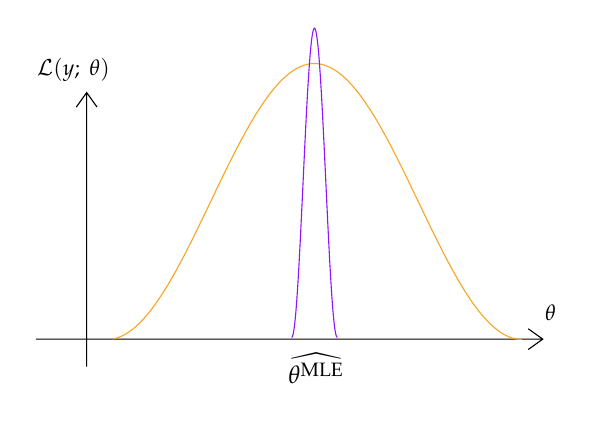
\begin{tikzpicture}[x=0.75pt,y=0.75pt,yscale=-1,xscale=1]
%uncomment if require: \path (0,300); %set diagram left start at 0, and has height of 300

%Shape: Axis 2D [id:dp33309643030277414] 
\draw  (48,169.8) -- (292.17,169.8)(72.42,51) -- (72.42,183) (285.17,164.8) -- (292.17,169.8) -- (285.17,174.8) (67.42,58) -- (72.42,51) -- (77.42,58)  ;
%Shape: Wave [id:dp761793702798415] 
\draw  [color={rgb, 255:red, 245; green, 166; blue, 35 }  ,draw opacity=1 ] (282.17,170) .. controls (264.07,170) and (248.47,137.57) .. (232.17,103.5) .. controls (215.86,69.43) and (200.26,37) .. (182.17,37) .. controls (164.07,37) and (148.47,69.43) .. (132.17,103.5) .. controls (116.77,135.67) and (102,166.38) .. (85.17,169.7) ;
%Shape: Wave [id:dp8411747217824341] 
\draw  [color={rgb, 255:red, 144; green, 19; blue, 254 }  ,draw opacity=1 ] (193.17,169) .. controls (191.18,169) and (189.46,132.67) .. (187.67,94.5) .. controls (185.87,56.33) and (184.16,20) .. (182.17,20) .. controls (180.18,20) and (178.46,56.33) .. (176.67,94.5) .. controls (174.87,132.67) and (173.16,169) .. (171.17,169) ;

% Text Node
\draw (183,184) node  [font=\small] [align=left] {$\displaystyle \widehat{\theta ^{\text{MLE}}}$};
% Text Node
\draw (296,157) node  [font=\footnotesize] [align=left] {$\displaystyle \theta $};
% Text Node
\draw (66,40) node  [font=\footnotesize] [align=left] {$\displaystyle \mathcal{L}( y;\ \theta )$};


\end{tikzpicture}

Clairement, la courbe \textcolor{purple}{en mauve} aura plus de points près de $\hat{\theta}^{\text{EMV}}$ que la courbe en \textcolor{orange}{orange}. On évalue cette différence avec la deuxième dérivée, soit la concavité ou \og curve \fg{}. Ce faisant, la deuxième dérivée permet d'être plus certain d'avoir le bon estimateur. Il est alors logique que la variance ne puisse pas être moins que l'estimateur du maximum de vraisemblance évalué au point où la concavité est maximisée. 

Finalement, on veut comprendre pourquoi $1/\text{\og curve \fg{}}$ et non juste $\text{\og curve \fg{}}$. On déduit que plus la concavité est élevée, alors plus la variance sera faible. Il aura forcément moins de points près de $\hat\theta^{\text{EMV}}$ et donc:
\begin{equation*}
	\text{Var}(\hat\theta^{\text{EMV}}) \overset{\text{dépend}}{\sim} \frac{1}{\text{\og curve \fg{}}}
\end{equation*}
On observe alors que la limite lorsque la \og curve \fg{} tend vers l'infini implique une variance nulle. On dit donc que la distribution de l'estimateur est "asymptotiquement normale" tel que $\hat\theta^{\text{EMV}} \overset{a.s.}{\rightarrow} \mathcal{N}\Big(\theta, \big(\bm{I}(\theta)\big)^{-1}\Big)$ où a.s. veut dire \hyperlink{asympto}{asymptotiquement}.

Il s'ensuit alors que \textbf{l'efficacité d'un estimateur} est le ratio de la borne Cramèr-Rao sur la variance de l'estimateur:
\begin{algo}{Efficacité d'un estimateur}
\begin{align*}
	\text{eff}(\theta)
	&=	\frac{\text{Var}(\hat{\theta})^{\text{Rao}}}{\text{Var}(\hat{\theta})} 
	=	\frac{1}{n\text{E}\left[\Big(\deriv{\theta}\ln f(x ; \theta)\Big)^{2}\right]\text{Var}(\hat{\theta})}
\end{align*}
\end{algo}

Si ce ratio est de 1, $\text{eff}(\theta) = 1$, alors l'estimateur est à la borne. On dit qu'il est un estimateur \og \textbf{efficient} \fg{} \textit{(angl.)}. Du fait, parmi les estimateurs sans biais il doit être celui avec la \textbf{variance minimale}; on dit que l'estimateur est le \og \textbf{Minimum Variance Unbiased Estimator (MVUE)} \fg{} \textit{(angl.)}. 

De plus, on peut généraliser cette formulation pour obtenir l'efficacité relative d'un estimateur comparativement à un autre:
\begin{algo}{Efficacité relative}
Soit les estimateurs non biaisés $\hat\theta_{n}$ et $\tilde\theta_{n}$, l'efficacité de $\hat\theta_{n}$ relativement à $\tilde\theta_{n}$ est:
\begin{align*}
	\text{eff}(\hat\theta_{n}, \tilde\theta_{n})
	&=	\frac{\text{Var}(\hat\theta_{n})}{\text{Var}(\tilde\theta_{n})}	
\end{align*}
\end{algo}
Si $\text{eff}(\hat\theta_{n}, \tilde\theta_{n}) < 1$ alors $\hat\theta_{n}$ est plus efficace et vice-versa.

Nous pouvons également évaluer si un estimateur est cohérent, ou converge, avec des très grands échantillons; un estimateur $\hat\theta$ est \textbf{consistent} \textit{(angl.)} si la probabilité qu'il diffère de la vraie valeur du paramètre $\theta$ par une erreur $\epsilon$ près de 0 tend vers 0 alors que la taille de l'échantillon $n$ tend vers l'infini:
\begin{algo}{Convergence (\textbf{consistency}) d'un estimateur}
\begin{align*}
	\underset{n \rightarrow \infty}{\lim} \Pr(\big| \hat\theta - \theta \big| > \epsilon) = 0, \quad \epsilon > 0
\end{align*}
\end{algo}

Ce critère peut être rencontré lorsque l'estimateur $\hat\theta$ est \hypertarget{asympto}{\textbf{asymptotiquement sans biais}} \textbf{\textit{et}} que la \textbf{variance de l'estimateur} tend vers 0. D'ailleurs, nous avons déjà raisonné ceci avec \hyperlink{cramer-rao}{la borne inférieure Cramèr-Rao}.


On définit proprement ce qu'est un estimateur \textbf{asymptotiquement sans biais}:
\begin{algo}{Estimateur asymptotiquement sans biais}
\begin{align*}
	\underset{n \rightarrow \infty}{\lim} \text{B}(\hat\theta) &= 0
\end{align*}
\end{algo}

Donc si $\underset{n \rightarrow \infty}{\lim} \text{Var}(\hat\theta) = 0$ et que $\underset{n \rightarrow \infty}{\lim} \text{B}(\hat\theta) = 0$ alors l'estimateur est \textbf{consistent}. 
Cependant, l'inverse n'est pas vrai; un estimateur qui est \textbf{consistent} n'implique pas que la variance et le biais tendent vers 0.

Malgré la nature plaisante de la convergence d'un estimateur, beaucoup d'estimateurs ont cette propriété. 
Nous voulons alors une mesure qui n'indique pas seulement qu'un estimateur arrive près de la bonne valeur souvent \textit{(alias, une très petite variance)}, mais qu'il est mieux que d'autres estimateurs.
De plus, dût à la sélection arbitraire de l'erreur $\epsilon$ pour la \textit{consistency} d'un estimateur, il est possible de malicieusement la sélectionner pour faire parler les données comme on le souhaite. 

Nous définissons alors l'\textbf{Erreur Quadratique Moyenne} (EQM), ou \textbf{Mean Squared Error (MSE)}, permettant de comparer les différents estimateurs ayant tous une bonne \textit{consistency} en assurant une cohérence d'interprétation.
\begin{algo}{Erreur Quadratique Moyenne (Mean Squared Error)}
\begin{align*}
	\text{MSE}_{\hat\theta}(\theta)
	&=	\text{E}[(\hat\theta - \theta)^{2} | \theta]
	\Leftrightarrow	\text{Var}(\hat\theta) + \left[\text{B}(\hat\theta)\right]^{2}
\end{align*}
\end{algo}

En combinant tous ces critères, le meilleur estimateur est alors l'estimateur \textbf{sans biais} ayant la \textbf{plus petite variance} possible parmi tous les estimateurs \textit{sans biais} possible; c'est-à-dire, le \textbf{Uniformly Minimum Variance Unbiased Estimator \textit{(UMVUE)}}.

\subsubsection*{Estimation par intervalles}

Un type d'estimateur par intervalle est l'\textbf{intervalle de confiance}:
\begin{algo}{Intervalle de confiance}
Soit le paramètre à estimer $\theta$, alors nous sommes confiants à un niveau de 100$(1 - \alpha)$\% qu'il est contenu entre $(L, U)$. 

De façon équivalente, nous sommes confiant à un seuil de $\alpha$\% qu'il est contenu entre $(L, U)$: 
\begin{equation*}
	\theta \in \left[ L, U\right].
\end{equation*}
Nous pouvons alors dire que $\Pr(L \le \theta \le U) \ge (1 - \alpha)$ pour tout $\theta$.
\end{algo}

Par exemple, dans le cas d'une population avec distribution normale et moyenne $\mu$ inconnue, on a la moyenne échantillonnale $\bar{x}$ (qui est l'estimateur \textit{MVUE}).
\begin{formula}{Intervalle de confiance sur la moyenne \textit{(distribution normale)}} 
Nous sommes confiants à un niveau de 100$(1 - \alpha)$\% que :
\begin{equation*}
	\mu \in \left[ \bar{x} - z_{\alpha/2} \frac{\sigma}{\sqrt{n}}, \bar{x} + z_{\alpha/2} \frac{\sigma}{\sqrt{n}}\right].
\end{equation*}
\end{formula}

%%%
%%%	Méthode du pivot
%%%

\subsection*{Construction d'estimateurs}

Dans la section précédente, on évalue les méthodes pour évaluer la \textbf{qualité} de l'estimateur. 
Cependant, comment obtenons-nous des estimateurs pour les évaluer?

Plusieurs méthodes existent pour établir des estimateurs, de plus plusieurs méthodes existent pour estimer des paramètres.
La méthode vu dans le cadre du cours de statistique est la \textbf{méthode fréquentiste}, le cours de mathématiques IARD 1 (ACT-2005) présente \textbf{l'estimation bayésienne}.

Avant de le faire, nous présentons quelques concepts:
\begin{description}
	\item[échantillon aléatoire:] Échantillon d'observations indépendantes provenant de la même distribution paramétrique (identiquement distribué); c'est-à-dire, un échantillon \textbf{(iid)}.
	\item[k-ème moment centré à 0:]  $\mu_{k}' = \text{E}[X^{k}]$.
	\item[$100g^{\text{ème}}$ pourcentile:]  $\pi_{g}(\theta) = F^{-1}_{\theta}(g)$.
\end{description}

Les deux premiers estimateurs ci-dessous sont les plus faciles à obtenir, mais sont aussi les moins performants puisqu'ils n'utilisent que quelques traits des données au lieu de l'entièreté des données comme la troisième méthode.

Cette distinction devient particulièrement importante dans le cas d'une distribution avec une queue lourde à la droite (Pareto, Weibull, etc.) où il devient plus essentiel de connaître les valeurs extrêmes pour bien estimer le paramètre de forme ($\alpha$ pour une Pareto).

Un autre désavantage est que les deux premières méthodes nécessitent que les données proviennent toutes de la même distribution, autrement les moments et quantiles ne seraient pas clairs.

Finalement, sous les deux premières méthodes la décision de quels moments et percentiles à utiliser est arbitraire.

\subsubsection*{Méthode des moments (MoM)}

Soit un échantillon aléatoire de taille $n$ (iid), on pose $\hat\mu_{k}' = \mu_{k}'$.
\begin{algo}{Estimation de $\theta$ par la méthode des moments}
L'estimation de $\theta$ est alors toute solution des $p$ équations:
\begin{equation*}
	\mu_{k}'(\theta) = \hat\mu_{k}', \quad	k = 1, 2, \dots, p
\end{equation*}
\end{algo}

La raison pour cet estimateur est que la distribution empirique aura les mêmes $p$ premiers moments centrés à 0 que la distribution paramétrique.

\subsubsection*{Méthode du \guillemotleft Percentile Matching \guillemotright}

Soit un échantillon aléatoire de taille $n$ (iid), on pose $\hat\pi_{g}(\theta) = \pi_{g}(\theta)$.

\begin{algo}{Estimation de $\theta$ par la méthode du \guillemotleft Percentile Matching \guillemotright}
L'estimation de $\theta$ est alors toute solution des $p$ équations:
\begin{equation*}
	F(\hat\pi_{g_{k}} | \theta)	=	g_{k}, \quad	k = 1, 2, \dots, p
\end{equation*}
\end{algo}

La raison pour cet estimateur est que le modèle produit aura $p$ percentiles qui vont \guillemotleft matcher \guillemotright les données.

Il peut arriver que les percentiles de distributions ne soient pas uniques, par exemple dans le cas de données discrètes lorsque le quantile recherché peut tomber entre 2 \emph{marches} de la fonction empirique, ou mal-définis.
Il est alors utile de définir une méthode d'interpolation des quantiles (bien qu'il n'en existe pas une d'officielle).

Soit le \guillemotleft \textbf{smoothed empirical estimate} \guillemotright d'un percentile:

\begin{algo}{Smoothed empirical estimate}
On utilise les statistiques d'ordre de l'échantillon $x_{(1)} \le x_{(2)} \le \dots \le x_{(n)}$ pour l'interpolation suivant:
\begin{align*}
	\hat\pi_{g}
	&=	(1 - h)x_{(j)} + h x_{(j + 1)}, \quad \text{ où }	\\
	j
	&=	\lfloor (n + 1) g \rfloor	&
	&\text{ et }	&
	h
	&=	(n + 1) g - j
\end{align*}
\end{algo}


\subsubsection*{Méthode du maximum de vraisemblance}

Nous cherchons à maximiser la probabilité d'observer les données.
Ceci est fait par la vraisemblance $\mathcal{L}(\theta; x)$ ou, puisque le logarithme ne change pas le maximum, la log-vraisemblance $\ell(\theta; x)$ où:

\begin{algo}{Maximum de vraisemblance}
\begin{align*}
	\mathcal{L}(\theta; x)
	&=	\prod_{i = 1}^{n}	f(x_{i}; \theta)	&
	&\text{et}	&
	\ell(\theta; x)
	&=	\sum_{i = 1}^{n} \ln	f(x_{i}; \theta)	&
\end{align*}
et l'\textbf{estimateur du maximum de vraisemblance} de $\bm\theta$ est celui qui maximise la fonction de vraisemblance.
\end{algo}

%%	Propriétés de l'EMV
%%		invariance, convergence, non-biais, Cramèr-Rao, ...

%\subsection*{Autres critères}
%	Quantile-Quantile
%	AIC
%	BIC

%%%
%%%
%%% pas pertinent au cours de stats %%%
%Cependant, il peut être pratique de généraliser cette fonction de vraisemblance pour les cas de données censurées ou tronquées.
%
%Soit un ensemble de données comportant n événements $A_{1}, \dots, A_{n}$ avec $A_{j}$ étant tout ce qui fut observé pour la $j^{\text{e}}$ observation; c'est-à-dire que $A_{j}$ pourrait être une observation unique ou un intervalle (par exemple, dans le cas de données groupées).
%
%De plus, un suppose que $A_{j}$ est une observation de la variable aléatoire $X_{j}$ et que les variables aléatoires $X_{1}, \dots, X_{n}$ ne doivent pas obligatoirement avoir la même distribution paramétrique; cependant, elles doivent tous dépendent du même vecteur paramétrique $\bm\theta$.
%Finalement, comme dans les deux autres cas, les variables aléatoires sont supposées indépendantes.
%
%\begin{align*}
%	\mathcal{L}(\theta; x)
%	&=	\prod_{j = 1}^{n}	\Pr(X_{j} \in A_{j} ; \theta)		
%\end{align*}
%
%Pour faire le lien avec la définition précédente, dans le cas où $A_{j}$ est un point unique et que la distribution est continue $\Pr(X_{j} \in A_{j} | \theta) = f(x_{i}; \theta)$.
%
%\begin{algo}{Données modifiées}
%Pour le cas de données groupées, les observations $c_{0} < c_{1} < \dots < c_{k}$ contiennent $n_{j}$ observations par intervalle $(c_{j - 1}, c_{j}]$, la fonction de vraisemblance est donc:
%\setlength{\mathindent}{-1cm}
%\begin{align*}
%	\mathcal{L}(\theta; x)
%	&=	\prod_{j = 1}^{n}	\left[ F(c_{j}|\theta) - F(c_{j-1}|\theta)\right]^{n_{j}},	\;	\text{données groupées}	\\
%	&=	\prod_{j = 1}^{n}	S(x_{i} ; \theta),	\;	\text{données censurées}	\\
%	&=	\prod_{j = 1}^{n}	\frac{f(x_{i}; \theta)}{S(x_{i} ; \theta)},	\;	\text{données tronquées}
%\end{align*}
%\setlength{\mathindent}{1cm}
%\end{algo}
%%% fin de pas pertinent au cours de stats %%%
%%%
%%%

%%%%%%%%	%%%%	%%%%	%%%%	%%%%	%%%%	%%%%	%%%%	%%%%	
%%%%		À rajouter éventuellement	%%%%	
%%%%%%%%	%%%%	%%%%	%%%%	%%%%	%%%%	%%%%	%%%%	%%%%	

%\subsection*{Tests d'hypothèses}
%%	Contenu à y inclure
%	Hypothèse nulle et alternative
%	Statistique de test
%	Région de réjection
%	Erreurs de type I et II
%		Tests optimaux
%		Lemme de Neymann-Pearson
%		Ratio de vraisemblance
%	Valeurs critique et seuil observé
%	Test unilatéral et bilatéral
%	La valeur p
%	
%	Test uniformément le plus puissant, alias Uniformely Most Powerful (UMP)
%	Tests échantillons normaux
%		Test T
%			Unilatéral (test, taille, puissance, seuil observé, IC)
%			Bilatéral (test, taille, puissance, seuil observé, IC)\\
%		Test sur la variance
%			3 différents problèmes (<=U<, >=U>, =U=/=)
%	Tests grands échantillons
%		Test Z (normal)
%			3 différents problèmes (<=U<, >=U>, =U=/=)
%			(tests, tailles, puissances, seuils observé, IC)
%	Test du Rapport de Vraisemblance
%		Statistique, test
%	Test d'adéquation
%		Fonction de répartition empirique
%		Test de Kolmogorov-Smirnov
%		Test du khi-carré de Pearson
%			design multinomial
%		Tableau de contingence
%		Test d'indépendance du khi-carré


%\subsection*{Distributions d'échantillonnage}
%%	Contenu à y inclure
%	Postulat de normalité
%		Moyenne échantillonnale
%		Variance échantillonnale
%		Statistique T
%		Statistique F
%	Échantillons de distribution inconnue
%		Théorème centrale limite

%\subsection*{Exhaustivité}
%%	Contenu à y inclure
%	Définition de l'exhaustivité
%	Théorème de factorisation de Fisher-Neymann
%	Critère de Lehmann-Scheffé (Exhaustivité minimale)
%	Théorème de factorisation de Fisher-Neymann (cas de plus d'un paramètre)
%	Théorème de Rao-Blackwell (statistique exhaustive sans biais)
%	MVUE
%		Élaboration sur le MVUE
%		Comment le construire

%%	Tableau des intervalles de confiance, tests d'hypothèses, etc. pour des cas spécifiques
%		Variance inconnue, moyenne inconnue pour une normale, proportion, petit échantillon, ...
\columnbreak	

\subsection*{Statistiques d'ordre}

Soit un échantillon aléatoire de taille $n$.
Nous définissons la \textbf{$k^{\text{e}}$ statistique d'ordre} $X_{(k)}$ comme étant la $k^{\text{e}}$ plus petite valeur d'un échantillon.\\
Les crochets sont utilisés pour différencier la $k^{\text{e}}$ statistique d'ordre $X_{(k)}$ de la $k^{\text{e}}$ observation $X_{k}$.\\

Nous sommes habituellement intéressés au minimum $X_{(1)}$ et le maximum $X_{(n)}$.

\setlength{\mathindent}{-0.75cm}
\begin{minipage}{0.5\columnwidth}
\begin{algo}{Minimum}
\begin{align*}
	X_{(1)}
	&=	\min(X_{1}, \dots, X_{n})	\\
	f_{X_{(1)}}(x)
	&=	n f_{X}(x) \big( S_{X}(x) \big)^{n - 1}	\\
	S_{X_{(1)}}(x)
	&=	\prod_{i = 1}^{n} \Pr(X_{i} > x)
\end{align*}
\end{algo}
\end{minipage}
\begin{minipage}{0.5\columnwidth}
\begin{algo}{Maximum}
\begin{align*}
	X_{(n)}
	&=	\max(X_{1}, \dots, X_{n})	\\
	f_{X_{(n)}}(x)
	&=	n f_{X}(x) \big( F_{X}(x) \big)^{n - 1}	\\
	F_{X_{(n)}}(x)
	&=	\prod_{i = 1}^{n} \Pr(X_{i} \le x)
\end{align*}
\end{algo}
\end{minipage}
\setlength{\mathindent}{1cm}

De façon plus générale, on défini:
\begin{algo}{$k^{\text{e}}$ statistique d'ordre}
\begin{align*}
%	X_{(k)}
	f_{X_{(k)}}(x)
	&=	\frac{n!}{\textcolor{teal}{(k - 1)!} \textcolor{cobalt}{1!} \textcolor{cyan}{(n - k)!}} \textcolor{teal}{\underset{\text{observations } < \ k}{\underbrace{\big[ F_{X}(x) \big]^{k - 1}}}} \textcolor{cobalt}{\overset{\text{observation } = \ k}{\overbrace{f_{X}(x)}}} \textcolor{cyan}{\underset{\text{observations } > \ k}{\underbrace{\big[ S_{X}(x) \big]^{n - k}}}} \\
	F_{X_{(k)}}(x)
	&=	\underset{\text{Probabilité qu'au moins } k \text{ des } n \text{ observations } X_{k} \text{ sont } \le \ x}{\underbrace{\sum_{i = 1}^{n} \binom{n}{i} [F_{X}(x)]^{j} [1 - F_{X}(x)]^{n - j}}}
\end{align*}
\end{algo}

Nous pouvons également définir quelques autres statistiques d'intérêt :

\begin{description}
	\item[$R = X_{(n)} - X_{(1)}$: ] \textbf{L'étendu}e (range) est la différence entre le minimum et le maximum d'un échantillon.
		\begin{itemize}[leftmargin = *]
		\item	L'utilité de l'étendue est limitée puisqu'elle est très sensible aux données extrêmes.
		\item	Par exemple, supposons qu’on observe des données historiques de température pour le 1er septembre. \\
				En moyenne, la température est de $16\degree C$, mais nous avons un cas extrême de $-60\degree C$ en 1745.\\
				L'étendue sera de $86\degree C$ ce qui n'est très représentatif des données.\\
				Donc, dans ce contexte, la mesure n'est pas d'une très grande utilité.
		\end{itemize}
	\item[$M = \frac{X_{(n)} + X_{(1)}}{2}$: ] \textbf{mi-étendue} (Midrange), est la moyenne entre le minimum et le maximum d'un échantillon.
		\begin{itemize}[leftmargin = *]
		\item	Pour comprendre ce que représente la mi-étendue, on la compare à la moyenne arithmétique.
		\item	La moyenne arithmétique considère les données observées et calcule leur moyenne.\\
				Il s'ensuit qu'elle ne considère pas les chiffres qui ne sont pas observés.
		\item	La mi-étendue considère \textbf{tous} les chiffres, observés ou non, entre la plus grande et la plus petite valeur d'un échantillon et en prend la moyenne.		
		\end{itemize}
\end{description}

\begin{conceptgen}{Exemple sur les statistiques d'ordre}
Soit un échantillon de données météorologiques $\{-30\degree, -24\degree, -7\degree, -23\degree, +5\degree\}$ (celsius).

Je suppose que ce sont des températures du 4 février observées lors des dernières années.
\begin{itemize}[leftmargin = *]
	\item	La moyenne arithmétique ($-22.25\degree C$) m'intéresse, car je peux savoir, en moyenne, ce qu'est la température le 4 février.
	\item	La mi-étendue ($-12.5\degree C$), tout comme l'étendue ($-35\degree C$), ne m'intéresse pas puisqu'elle ne prend pas en considération la vraisemblance des différentes températures.
\end{itemize}

Maintenant, je suppose que ces données sont des températures observées tout au long de l'hiver passé.
\begin{itemize}[leftmargin = *]
	\item	La moyenne arithmétique ne m'intéresse pas puisqu'elle est beaucoup trop biaisée par les températures de cette même journée. 
	\item	Cependant, la mi-étendue et l'étendue me donnent maintenant une meilleure idée de la température de l'hiver.
\end{itemize}

L'important à retenir est que l'utilité des mesures dépend de la situation. Également, ceci est un exemple \textbf{très} simpliste et dans tous les cas on ne peut pas tirer de conclusions sur les températures de l'hiver à partir d'une seule journée.
\end{conceptgen}

Nous pouvons définir la \textbf{médiane} en termes de statistiques d'ordre:
\begin{align*}
	\text{Med}
	&=	\left\{
		\begin{matrix}
			X_{((n + 1)/2)},		&	\text{si n est impair}	\\
			\frac{X_{(n/2)} + X_{(n/2 + 1)}}{2},	&	\text{si n est pair}	\\
		\end{matrix}
	\right.
\end{align*}

Finalement, on définit la distribution conjointe du minimum et du maximum $\forall x < y$:
\begin{align*}
	f_{X_{(1)}, X_{(n)}}(x, y)
	&=	n (n - 1) [F_{X}(y) - F_{X}(x)]^{n - 2} f_{X}(x) f_{X}(y)
\end{align*}

\pagebreak

\section*{Modèles linéaires en actuariat}

\subsection*{Régression linéaire simple}

\begin{definitionNOHFILL}[Modèle de régression linéaire simple]
\begin{align*}
	Y_{i} 
	&=	\beta_{0} + \beta_{1} x_{i} + \varepsilon_{i}
\end{align*}
\end{definitionNOHFILL}

\subsubsection*{Exemple de compréhension}

On illustre le concept et la signification des paramètres de régression avec cet exemple illustratif

\paragraph{Objectif}	On veut deviner le coût d'une télévision (télé) selon la taille de son écran.

\

L'idée de la "régression" est de deviner, ou "prédire" du mieux qu'on peut le coût d'une télé en fonction de la taille de son écran.

Deviner le coût \textit{exact} d'une télé \textit{seulement} en fonction de la taille de son écran est impossible. Il y a de nombreuses raisons qui déterminent le prix d'une télé et un bon exercice est de réfléchir à ce qu'elles pourraient être. 
J'inclus ci-dessous une liste de quelques raisons, ou "facteurs", qui me sont survenus:
\begin{itemize}[leftmargin = *]
	\item	La compagnie qui la produit (Sony vs LG, etc.).
	\item	La résolution (4K vs 360p).
	\item	L'année de fabrication (1990 vs 2020).
	\item	L'endroit de l'achat (Amazon vs BestBuy, Mexique vs Canada, etc.).
	\item	Le temps de l'année (été vs hiver, Boxing Day, etc.).
\end{itemize}

Maintenant supposons que tu joues à un jeu avec tes amis où qu'ils doivent deviner le coût d'une télé en fonction de sa taille. Ils vont probablement tous te donner des différentes réponses.

Si tu crées un modèle de prévision, il doit être systématique et toujours deviner le même prix pour la même taille d'écran---même si la prévision est erronée. 

Alors, supposons que tu changes le jeu un peu et stipules que la personne qui devine le prix le plus éloigné doit prendre une gorgée de sa bière. Les réponses de tes amis vont probablement se ressembler un peu plus, mais il y a un problème qui demeure---tu veux que les prévisions soient proportionnelles à la taille de l'écran. C'est-à-dire, si ton ami devine qu'une télé de 25" coûte 100\$, tu t'attends à ce qu'il devine qu'une télé de 50" coûte 200\$.

La raison est qu'une régression \textbf{linéaire} \textit{simple} est simplement une ligne droite:
\begin{center}

\tikzset{every picture/.style={line width=0.75pt}} %set default line width to 0.75pt        

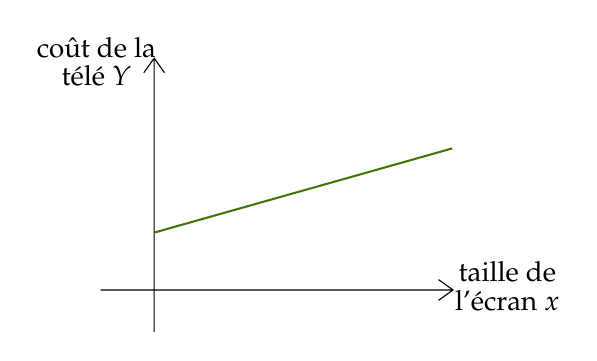
\begin{tikzpicture}[x=0.75pt,y=0.75pt,yscale=-1,xscale=1]
%uncomment if require: \path (0,300); %set diagram left start at 0, and has height of 300

%Shape: Axis 2D [id:dp3720388407437436] 
\draw  (50,144.67) -- (219.83,144.67)(75.83,33) -- (75.83,165) (212.83,139.67) -- (219.83,144.67) -- (212.83,149.67) (70.83,40) -- (75.83,33) -- (80.83,40)  ;
%Straight Lines [id:da45260329028360524] 
\draw [color={rgb, 255:red, 65; green, 117; blue, 5 }  ,draw opacity=1 ][line width=0.75]    (76.05,116.98) -- (219.41,76.48) ;

% Text Node
\draw (246,142.67) node   [align=left] {\shortstack{taille de\\ l'écran $x$}};
% Text Node
\draw (48,34.67) node   [align=left] {\shortstack{coût de la \\ télé $Y$}};


\end{tikzpicture}

\end{center}

L'intuition est que ton ami se base uniquement sur la taille de l'écran comme information pour deviner le coût. Une régression \textbf{linéaire} simple applique un facteur \textbf{multiplicatif}. Il ne peut pas se dire que plus grand l'écran est grand, plus le prix va augmenter---ceci serait plutôt une régression avec un paramètre \textbf{exponentiel}. 

On crée donc un facteur surnommé "paramètre". Dans le cas d'une régression linéaire simple, on a deux paramètres d'intérêts: un "niveau de base" pour le coût $\beta_{0}$ et un "multiplicateur" de la taille d'écran $\beta_{1}$:
\begin{center}
\tikzset{every picture/.style={line width=0.75pt}} %set default line width to 0.75pt        

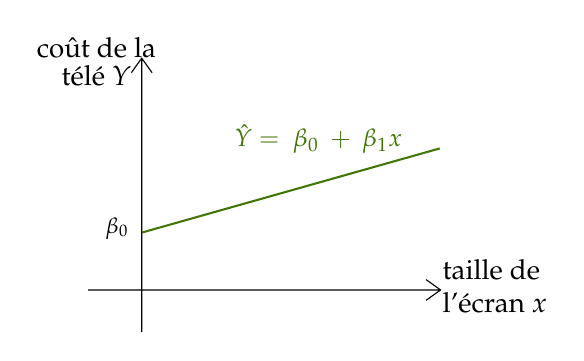
\begin{tikzpicture}[x=0.75pt,y=0.75pt,yscale=-1,xscale=1]
%uncomment if require: \path (0,300); %set diagram left start at 0, and has height of 300

%Shape: Axis 2D [id:dp3720388407437436] 
\draw  (50,144.67) -- (219.83,144.67)(75.83,33) -- (75.83,165) (212.83,139.67) -- (219.83,144.67) -- (212.83,149.67) (70.83,40) -- (75.83,33) -- (80.83,40)  ;
%Straight Lines [id:da45260329028360524] 
\draw [color={rgb, 255:red, 65; green, 117; blue, 5 }  ,draw opacity=1 ][line width=0.75]    (76.05,116.98) -- (219.41,76.48) ;

% Text Node
\draw (246,142.67) node   [align=left] {taille de\\ l'écran $x$};
% Text Node
\draw (54,34.67) node   [align=left] {\shortstack{coût de la \\ télé $Y$}};

% Text Node
\draw (64,115) node  [font=\footnotesize] [align=left] {$\beta _{0}$};
% Text Node
\draw (161,72) node  [font=\small,color={rgb, 255:red, 65; green, 117; blue, 5 }  ,opacity=1 ] [align=left] {$\hat{Y} =\ \beta _{0} \ +\ \beta _{1} x$};


\end{tikzpicture}

\end{center}

On suppose qu'une télé doit coûter au moins un certain prix. Ce "niveau de base" est l'intercepte sur le graphique ci-dessus surnommé l'ordonnée $\beta_{0}$. De ton gré, tu supposes au moins $\beta_{0} = 200\$$ pour cet exemple. 

Ensuite, le multiplicateur va multiplier la taille de l'écran pour obtenir un prix. Ce paramètre représente donc la pente $\beta_{1}$. De ton gré, tu suppose une pente de $\beta_{1} = 2\$$ pour cet exemple. 

Le coût (l'axe des $Y$) est la variable qui dépend de la taille---c'est la variable "dépendante" $Y$. La taille (l'axe des $x$) est la variable que l'on connaît indépendamment du coût---c'est la variable "indépendante" $x$. 

Finalement la droite elle-même est le coût que le modèle devine $\hat{Y}$. Le chapeau signifie que c'est une estimation, ou "prévision".

Par exemple, le modèle devine que le prix d'une télé de 50" est de 300\$; soit, $\hat{Y} = \beta_{0} + \beta_{1} x = 200 + (2) \cdot (50) = 300$. Selon le modèle, on estime que le coût de la télé est de 300\$.

Maintenant, si tu connais le \textit{vrai} coût réel $Y$ tu peux mesurer à quel point tu est dans le champ. Supposons que le vrai coût est de $Y = 400\$$. Alors, l'erreur dans ta prédiction est de $\varepsilon = 400 - 300 = 100\$$. 

Graphiquement:


\tikzset{every picture/.style={line width=0.75pt}} %set default line width to 0.75pt        

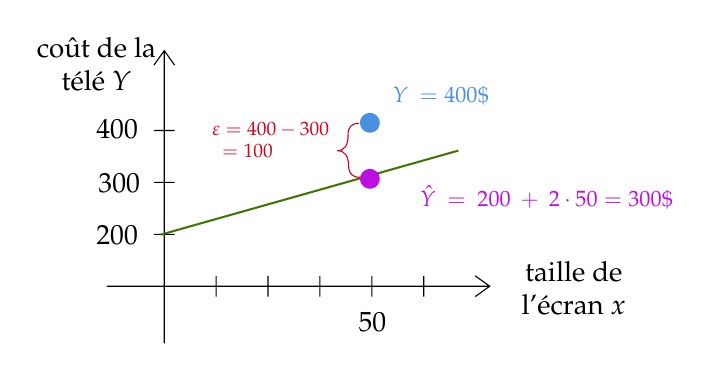
\begin{tikzpicture}[x=0.75pt,y=0.75pt,yscale=-1,xscale=1]
%uncomment if require: \path (0,300); %set diagram left start at 0, and has height of 300

%Shape: Axis 2D [id:dp0590336014536994] 
\draw  (50,141.82) -- (234.5,141.82)(77.7,28.33) -- (77.7,169.33) (227.5,136.82) -- (234.5,141.82) -- (227.5,146.82) (72.7,35.33) -- (77.7,28.33) -- (82.7,35.33) (102.7,136.82) -- (102.7,146.82)(127.7,136.82) -- (127.7,146.82)(152.7,136.82) -- (152.7,146.82)(177.7,136.82) -- (177.7,146.82)(202.7,136.82) -- (202.7,146.82)(72.7,116.82) -- (82.7,116.82)(72.7,91.82) -- (82.7,91.82)(72.7,66.82) -- (82.7,66.82) ;
\draw   ;
%Straight Lines [id:da6064475343931128] 
\draw [color={rgb, 255:red, 65; green, 117; blue, 5 }  ,draw opacity=1 ][line width=0.75]    (76.05,116.98) -- (219.41,76.48) ;
%Flowchart: Connector [id:dp8477117117153217] 
\draw  [draw opacity=0][fill={rgb, 255:red, 189; green, 16; blue, 224 }  ,fill opacity=1 ][line width=3]  (173.73,93.81) .. controls (171.68,92.14) and (171.38,89.12) .. (173.05,87.07) .. controls (174.72,85.02) and (177.74,84.71) .. (179.79,86.39) .. controls (181.84,88.06) and (182.15,91.08) .. (180.48,93.13) .. controls (178.8,95.18) and (175.79,95.49) .. (173.73,93.81) -- cycle ;
%Flowchart: Connector [id:dp4707804099581703] 
\draw  [draw opacity=0][fill={rgb, 255:red, 74; green, 144; blue, 226 }  ,fill opacity=1 ][line width=3]  (173.73,66.81) .. controls (171.68,65.14) and (171.38,62.12) .. (173.05,60.07) .. controls (174.72,58.02) and (177.74,57.71) .. (179.79,59.39) .. controls (181.84,61.06) and (182.15,64.08) .. (180.48,66.13) .. controls (178.8,68.18) and (175.79,68.49) .. (173.73,66.81) -- cycle ;
%Shape: Brace [id:dp37242003440355953] 
\draw  [color={rgb, 255:red, 208; green, 2; blue, 27 }  ,draw opacity=1 ] (171.5,63.33) .. controls (167.93,63.4) and (166.18,65.22) .. (166.25,68.79) -- (166.25,68.79) .. controls (166.35,73.89) and (164.61,76.47) .. (161.04,76.54) .. controls (164.61,76.47) and (166.45,78.99) .. (166.54,84.08)(166.5,81.79) -- (166.54,84.08) .. controls (166.61,87.65) and (168.43,89.4) .. (172,89.33) ;

% Text Node
\draw (275,142.67) node   [align=center] {taille de\\ l'écran $x$};
% Text Node
\draw (45,34.67) node   [align=center] {coût de la \\ télé $Y$};

% Text Node
\draw (262,99) node  [font=\footnotesize,color={rgb, 255:red, 189; green, 16; blue, 224 }  ,opacity=1 ] [align=left] {$\displaystyle \hat{Y} \ =\ 200\ +\ 2\cdot 50=300\$$};
% Text Node
\draw (55,117.33) node   [align=left] {$\displaystyle 200$};
% Text Node
\draw (56,92.33) node   [align=left] {$\displaystyle 300$};
% Text Node
\draw (55,66.33) node   [align=left] {$\displaystyle 400$};
% Text Node
\draw (211,50) node  [font=\footnotesize,color={rgb, 255:red, 74; green, 144; blue, 226 }  ,opacity=1 ] [align=left] {$\displaystyle Y\ =400\$$};
% Text Node
\draw (129,72.33) node  [font=\scriptsize,color={rgb, 255:red, 208; green, 2; blue, 27 }  ,opacity=1 ] [align=left] {$\displaystyle  \begin{array}{{>{\displaystyle}l}}
\varepsilon =400-300\\
\ \ =100
\end{array}$};
% Text Node
\draw (178,159.33) node   [align=left] {$\displaystyle 50$};


\end{tikzpicture}

On voit donc que $Y = \beta_{0} + \beta_{1} x + \varepsilon$ est un "modèle" théorique pour obtenir une variable dépendante $Y$ en fonction de: 
\begin{itemize}
	\item	Une variable indépendante $x$ multipliée par un facteur $\beta_{1}$.
	\item	Un niveau de base l'intercepte $\beta_{0}$.
	\item	Une erreur aléatoire $\varepsilon$ inconnue.
\end{itemize}

\end{multicols*}

\end{document}
